\documentclass[a4paper]{article}

\usepackage[spanish]{babel}
\usepackage{graphicx}
\usepackage{amsmath, amssymb}
\usepackage[margin=2cm]{geometry}
\usepackage{fancyhdr}
\usepackage{enumerate}
\usepackage[shortlabels]{enumitem}
\usepackage{parskip}
\usepackage[most]{tcolorbox}
\usepackage[hidelinks]{hyperref}
\usepackage{float}


% cabecera
\pagestyle{fancy}
\fancyhead[l]{Daniel Soto}
\fancyhead[c]{Problemas de Astronomía \#8}
\fancyhead[r]{\today}
\fancyfoot[c]{\thepage}
\renewcommand{\headrulewidth}{0.2pt} % linea horizontal

%% Definicion de comandos para formato de unidades fisicas %%
\newcommand{\m}{\text{m}}
\newcommand{\cm}{\text{cm}}
\newcommand{\km}{\text{km}}
\newcommand{\s}{\text{s}}
\newcommand{\N}{\text{N}}
\newcommand{\g}{\text{g}}
\newcommand{\kg}{\text{kg}}
\newcommand{\Msolar}{\text{M}_\odot}
\newcommand{\Mterrestre}{\text{\text{M}_\oplus}}
\newcommand{\AU}{\text{AU}}
\newcommand{\ly}{\text{ly}}
\newcommand{\nT}{\text{nT}}
\newcommand{\GeV}{\text{GeV}}
\newcommand{\atomscm}{\text{atoms/cm}^3}
\newcommand{\K}{\text{K}}
\newcommand{\J}{\text{J}}
\newcommand{\My}{\text{My}}


\newcounter{problema}

\newtcolorbox[use counter=problema]{problema}[1][]{%
	breakable,
    colback=gray!15,
    colframe=gray!60,
    fonttitle=\bfseries,
    title={Problema~\theproblema:},
    boxrule=0.5mm,
    arc=3mm,
    boxsep=5pt,
    left=8pt,
    right=8pt,
    top=6pt,
    bottom=6pt,
    #1
}


\begin{document}

\begin{problema}

    \begin{figure}[H]
        \centering
        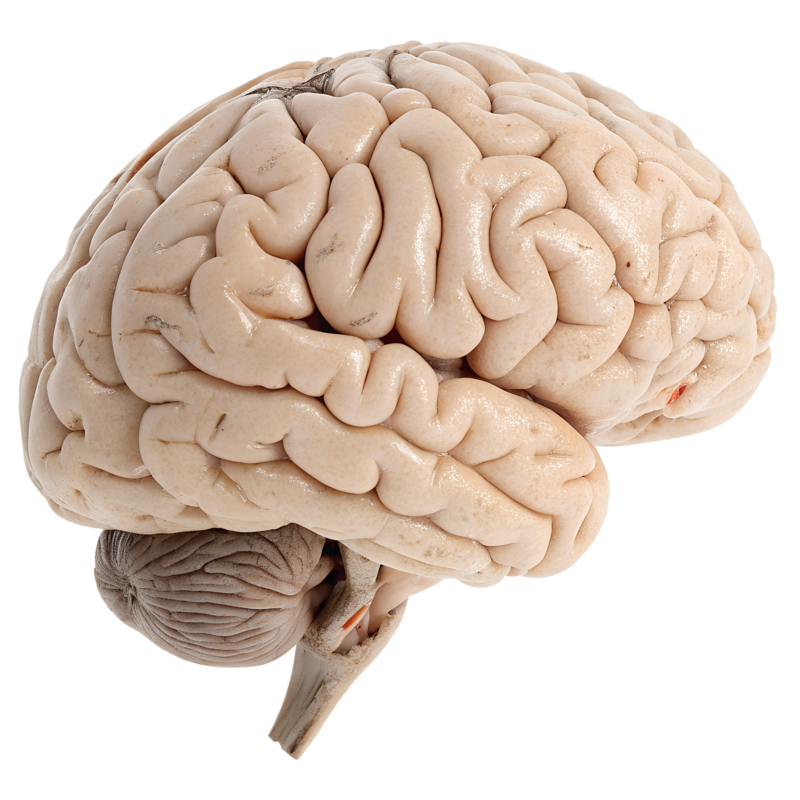
\includegraphics[width=0.4\textwidth]{Brain.png}
        \caption{Cerebro Humano}
        \label{fig:1}
    \end{figure}

\textbf{La Evolución de la Inteligencia:} La encefalización es una medida del tamaño del cerebro de un mamífero en comparación con su masa corporal. 
Aunque los cuerpos grandes a menudo requieren cerebros proporcionalmente más grandes para operar todos sus sistemas, la encefalización se considera una medida 
del tamaño "excesivo" del cerebro y, por tanto, una medida indirecta de la inteligencia bruta de una especie de mamífero. 
La tabla siguiente muestra el \textit{cociente de encefalización} (EQ) para algunos mamíferos comunes, junto con la edad de la especie.

\begin{table}[H]
\centering
\begin{tabular}{|l|c|c|c|c|}
\hline
\textbf{Especie} & \textbf{Edad ($\My$)} & \textbf{EQ} & \textbf{Tamaño Poblacional} & \textbf{Genes} \\
\hline
Humano            & 1       & 7.5 & 6 mil millones & 24000 \\
\hline
Delfín             & 50      & 4.1 & 600 000        & 24000 \\
\hline
Orca               & 70      & 2.7 & 5 000          & 20000 \\
\hline
Chimpancé          & 10      & 2.3 & 150 000        & 19700 \\
\hline
Perro              & 40      & 1.2 & 300 millones   & 19300 \\
\hline
Gato               & 12      & 1.0 & 200 millones   & 20285 \\
\hline
Caballo            & 50      & 0.9 & 58 millones    & 20436 \\
\hline
Rata               & 80      & 0.4 & 4 mil millones & 23 000 \\
\hline
\end{tabular}
\caption{Encefalización a través el tiempo.}
\label{tab:1}
\end{table}

\begin{enumerate}
	\item Grafica el EQ en función del tiempo. ¿Cuál es la tasa promedio de aumento del EQ por cada 10 millones de años hasta la época actual?

	\item ¿Cuántos años tomará para que el EQ se duplique?

	\item ¿Existe alguna tendencia entre: 
	\begin{enumerate}
		\item El EQ y el número de genes en la especie? 
		\item El EQ y el tamaño de la población de la especie? 
		\item El EQ y la edad de la especie?
	\end{enumerate}

	\item Se ha estimado que la tasa promedio de mutación genética en mamíferos es de $2.2 \times 10^{-9} \text{ Mutations / per nucleotide / year}$. 
	El tamaño promedio del genoma para las especies de mamíferos anteriores es de aproximadamente 3 mil millones, de los cuales el $3\%$ corresponde a genes que codifican proteínas. 
	\begin{enumerate}
		\item  ¿Aproximadamente cuántas mutaciones distinguen a una rata de un humano? 
		\item  ¿Cuántas mutaciones estarían presentes en el material genético?
	\end{enumerate}
\end{enumerate}

        


    
\end{problema}
[13] \cite{NASA_AstrobiologyMath}

\begin{problema}
\textbf{Determinantes genéticos de la inteligencia de las especies:} La tabla de abajo presenta los genes que han desempeñado un papel en el desarrollo de la inteligencia avanzada en la Tierra. 
Las mutaciones en cualquiera de estos genes causan problemas conocidos de desarrollo cerebral.
Para que la evolución en la Tierra condujera a una inteligencia avanzada, tamaños cerebrales más grandes y habilidades de comunicación fueron un requisito básico, 
además de capacidades para recordar detalles, aprender y emplear habilidades de pensamiento avanzadas. 
Todos estos atributos fueron posibles gracias a la activación de genes específicos en el genoma mamífero.
En un mundo alienígena, se asume que genes similares que afectan el alcance y la complejidad de los sistemas nerviosos también desempeñan un papel.
El genoma mamífero tiene aproximadamente 3 mil millones de nucleótidos de longitud. En los humanos, solo el $3\%$ está en forma de genes que codifican proteínas. 
El número total de genes mamíferos es de aproximadamente 24 000 para la mayoría de las especies. 
El significativo aumento en la inteligencia animal ocurrió cuando la Tierra había desarrollado una biosfera con decenas de millones de especies animales.
Este dramático aumento en la inteligencia ocurrió durante los últimos 50 millones de años (mamíferos avanzados), 
y más espectacularmente durante el último millón de años (como Homo Sapiens, Homo Neanderthalensis, Homo Heidelbergensis, etc.).

\begin{table}[H]
\centering
\begin{tabular}{|l|c|l|}
\hline
\textbf{Gen} & \textbf{Tamaño} & \textbf{Funciones} \\
\hline
FOX P2       & 607463         & Producción y comprensión del habla \\
\hline
Beta Catenin & 23200          & Tamaño del cerebro \\
\hline
Pax-6        & 33170          & Formación del ojo \\
\hline
Otoferlin    & 101496         & Audición \\
\hline
RGS-14       & 14756          & Aprendizaje, memoria \\
\hline
SIRT-1       & 33721          & Memoria, aprendizaje, afrontamiento \\
\hline
COMT        & 28236          & Habilidades de pensamiento \\
\hline
KRTHAP-1     & 6658           & Crecimiento del cabello \\
\hline
Myh-16       & 24672          & Tamaño de la mandíbula y volumen del cráneo \\
\hline
FGF-5        & 24430          & Longitud del cabello \\
\hline
ASPM         & 62568          & Crecimiento de la corteza cerebral \\
\hline
MSX-2        & 6328           & Sincronía entre cerebro y cráneo \\
\hline
FGFR-3       & 15461          & Crecimiento de cerebro y cráneo \\
\hline
TWIST        & 2205           & Crecimiento de cerebro y cráneo \\
\hline
DTNBP-1      & 140258         & Resolución de problemas, aprendizaje, comprensión \\
\hline
\end{tabular}
\caption{Genes involucrados en el desarrollo de la inteligencia avanzada en mamíferos.}
\label{tab:genes_inteligencia}
\end{table}

\begin{enumerate}
	\item ¿Qué porcentaje de los genes mamíferos están aparentemente involucrados en sentar las bases para el desarrollo futuro de la inteligencia avanzada?

	\item El número total de especies animales es de aproximadamente 2 millones. ¿Qué porcentaje logró una inteligencia avanzada después de 600 millones de años de evolución?

	\item Explica cómo la competencia interespecífica puede llevar a que, en cualquier momento dado, solo una especie sobreviviente con inteligencia avanzada viva en un planeta.
\end{enumerate}

\end{problema}
[14] \cite{NASA_AstrobiologyMath}

\begin{problema}
\textbf{Cataclismos Naturales y Evolución de las Especies:}  Los científicos han retomado recientemente la antigua idea de que la evolución de la vida a menudo está determinada por cataclismos naturales. 
Estos eventos son aleatorios en su naturaleza, pero representan un desafío mayor para las especies que deben sobrevivir a ellos. 
Muchos no lo logran, como podemos ver en las numerosas \textit{Extinciones Masivas} que han ocurrido. 
Uno podría preguntarse legítimamente cómo otros sistemas planetarios pueden haber tenido múltiples episodios de origen de la vida, pero algunos cataclismos detuvieron la evolución en su camino.

    \begin{figure}[H]
        \centering
        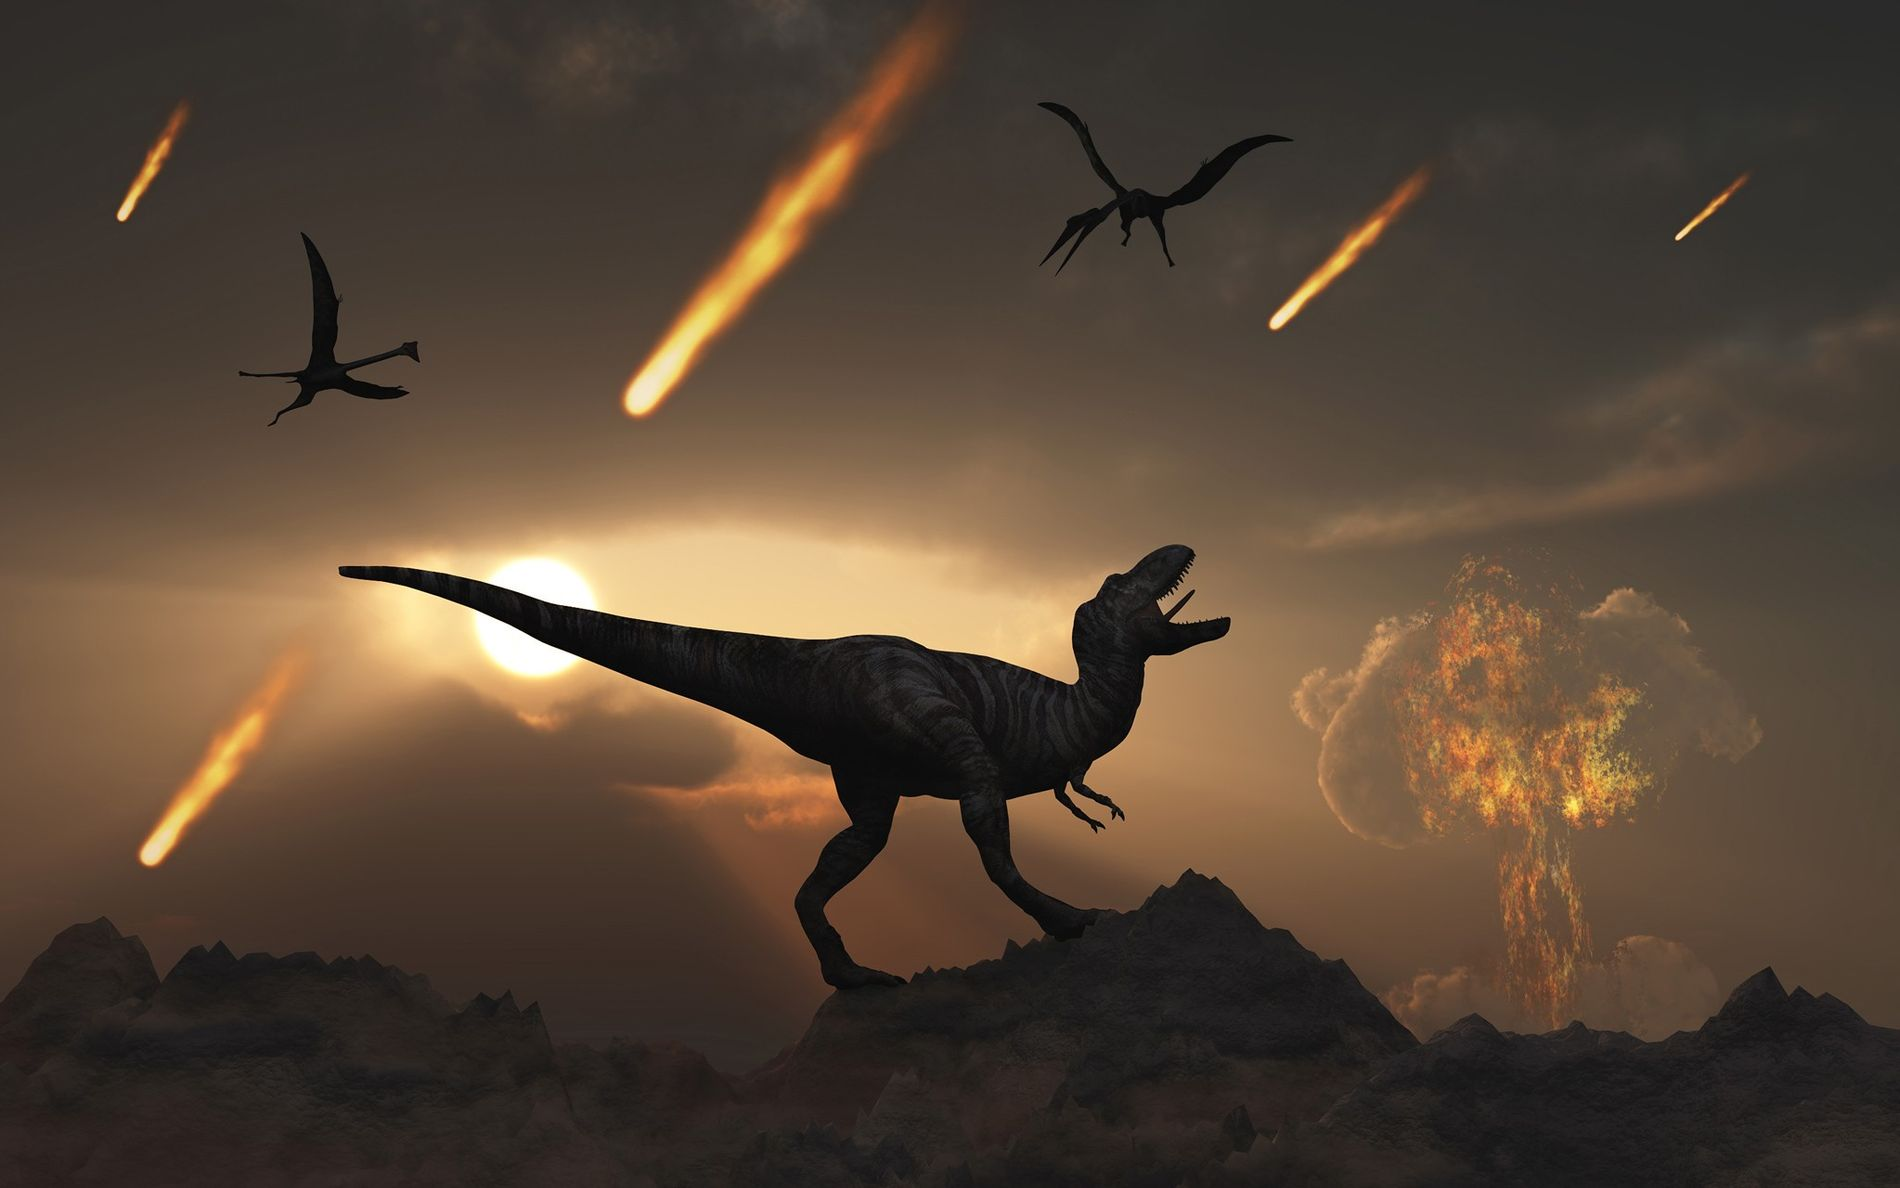
\includegraphics[width=0.7\textwidth]{Cataclysm.jpg}
        %\caption{}
        \label{fig:1}
    \end{figure}


Debemos recordar que, en la Tierra, más del $99\%$ de todas las especies que han existido alguna vez están extintas.

\begin{table}[H]
\centering
\begin{tabular}{|l|c|l|}
\hline
\textbf{Evento} & \textbf{Tiempo (millones de años)} & \textbf{Consecuencia} \\
\hline
Erupción Volcánica Toba & 0.07 & Cuello de botella en la evolución humana \\
\hline
Calentamiento Global & 55 & Extinción Paleoceno \\
\hline
Impacto de Asteroide & 65 & Extinción de los dinosaurios \\
\hline
Enfriamiento Global & 205 & Extinciones Triásico-Jurásicas \\
\hline
Calentamiento Global & 251 & Extinciones Pérmico-Triásicas \\
\hline
Enfriamiento Global & 370 & Extinciones Devónico Tardío \\
\hline
Enfriamiento Global & 440 & Extinciones Ordovícicas \\
\hline
Anoxia Oceánica & 540 & Extinción Ediacárica Final \\
\hline
Enfriamiento Global & 650 & Tierra de Bola de Nieve \\
\hline
\end{tabular}
\caption{Eventos de extinción conocidos o sospechados y sus consecuencias.}
\label{tab:3}
\end{table}

Los científicos en su mayoría coinciden en que los \textit{Eventos de Nivel de Extinción} (ELEs) requieren que un asteroide o cometa de gran tamaño colisione con la Tierra, 
y que sus dimensiones deben ser de al menos 5 kilómetros para generar suficiente energía cinética y afectar gravemente la biosfera global. 
La Tierra se encuentra cómodamente lejos de la mayor concentración de asteroides en el sistema solar; el Cinturón de Asteroides. 
Sin embargo, Marte es un planeta potencialmente habitable muy cercano al Cinturón de Asteroides. 
No es difícil imaginar que Marte reciba muchos más impactos importantes que la Tierra. 
También existen otras calamidades naturales que pueden causar extinciones, como episodios incrementados de actividad volcánica, 
generación de calentamiento global o la migración de los continentes que provocan cambios climáticos y ecológicos durante millones de años.


\begin{enumerate}
	\item A partir de la tabla, ¿cuál es aproximadamente el tiempo promedio entre los principales eventos de extinción en la Tierra?

	\item Un asteroide esférico de 10 kilómetros de diámetro choca contra la Tierra a una velocidad de $v = 20000 \m/\s$. 
	Si el asteroide está hecho de material rocoso, su masa podría ser de $m = 2 \times 10^{15} \kg$. 
	Si su energía cinética, en $\J$, viene dada por la fórmula
	$$E_k = \frac{1}{2}mv^2$$
	y una erupción solar típica produce unos $10^{23} \J$ de energía, 
	¿cuánta energía libera un impacto de asteroide en comparación con una erupción solar típica?
\end{enumerate}

\end{problema}
[15] \cite{NASA_AstrobiologyMath}


\bibliographystyle{plainurl}
\bibliography{bibliografia} % Nombre del .bib

\end{document}
